\section{Results}

\subsection{\textit{Laboea strobila} automated image classification}

Automated classification performs remarkably well for the ciliate, {Laboea strobila}. For this organism, the classifier has a probability of detection = 0.97 and precision = 0.90 before application of any score threshold. With the selected score threshold of 0.7, the corresponding probability of detection drops to 0.79 (19\% unclassified and 2\% misclassified), while the precision increases to 0.99.

\subsection{\textit{Laboea strobila} seasonality}

The oligotrich, Laboea strobila, displays a strong annual systematic seasonality. Peaks in daily-binned biomass occur regularly in the spring, reaching maximum yearly biomass no earlier than April 10th (2010) and no later than May 31st (2003) with the exception of a narrow peak in biomass on June 12, 2011. Peak biomass ranges from (  to  ). To a more varying degree of occurrence, timing, and amplitude, Laboea strobila exhibits a second peak of biomass in the fall (dates and peaks ranging from). 

\subsection{\textit{Laboea strobila} interannual variability}

\subsection{\textit{Laboea strobila} and environmental effects}

\subsection{\textit{Laboea strobila} interactions with 2-10 $\upmu$m eukaryote decrease}



\section{Discussion}

Discussion text

\newpage
\begin{figure}
%\vspace{2.4in}

\graphicspath{ {Chapter3_Figures/} }
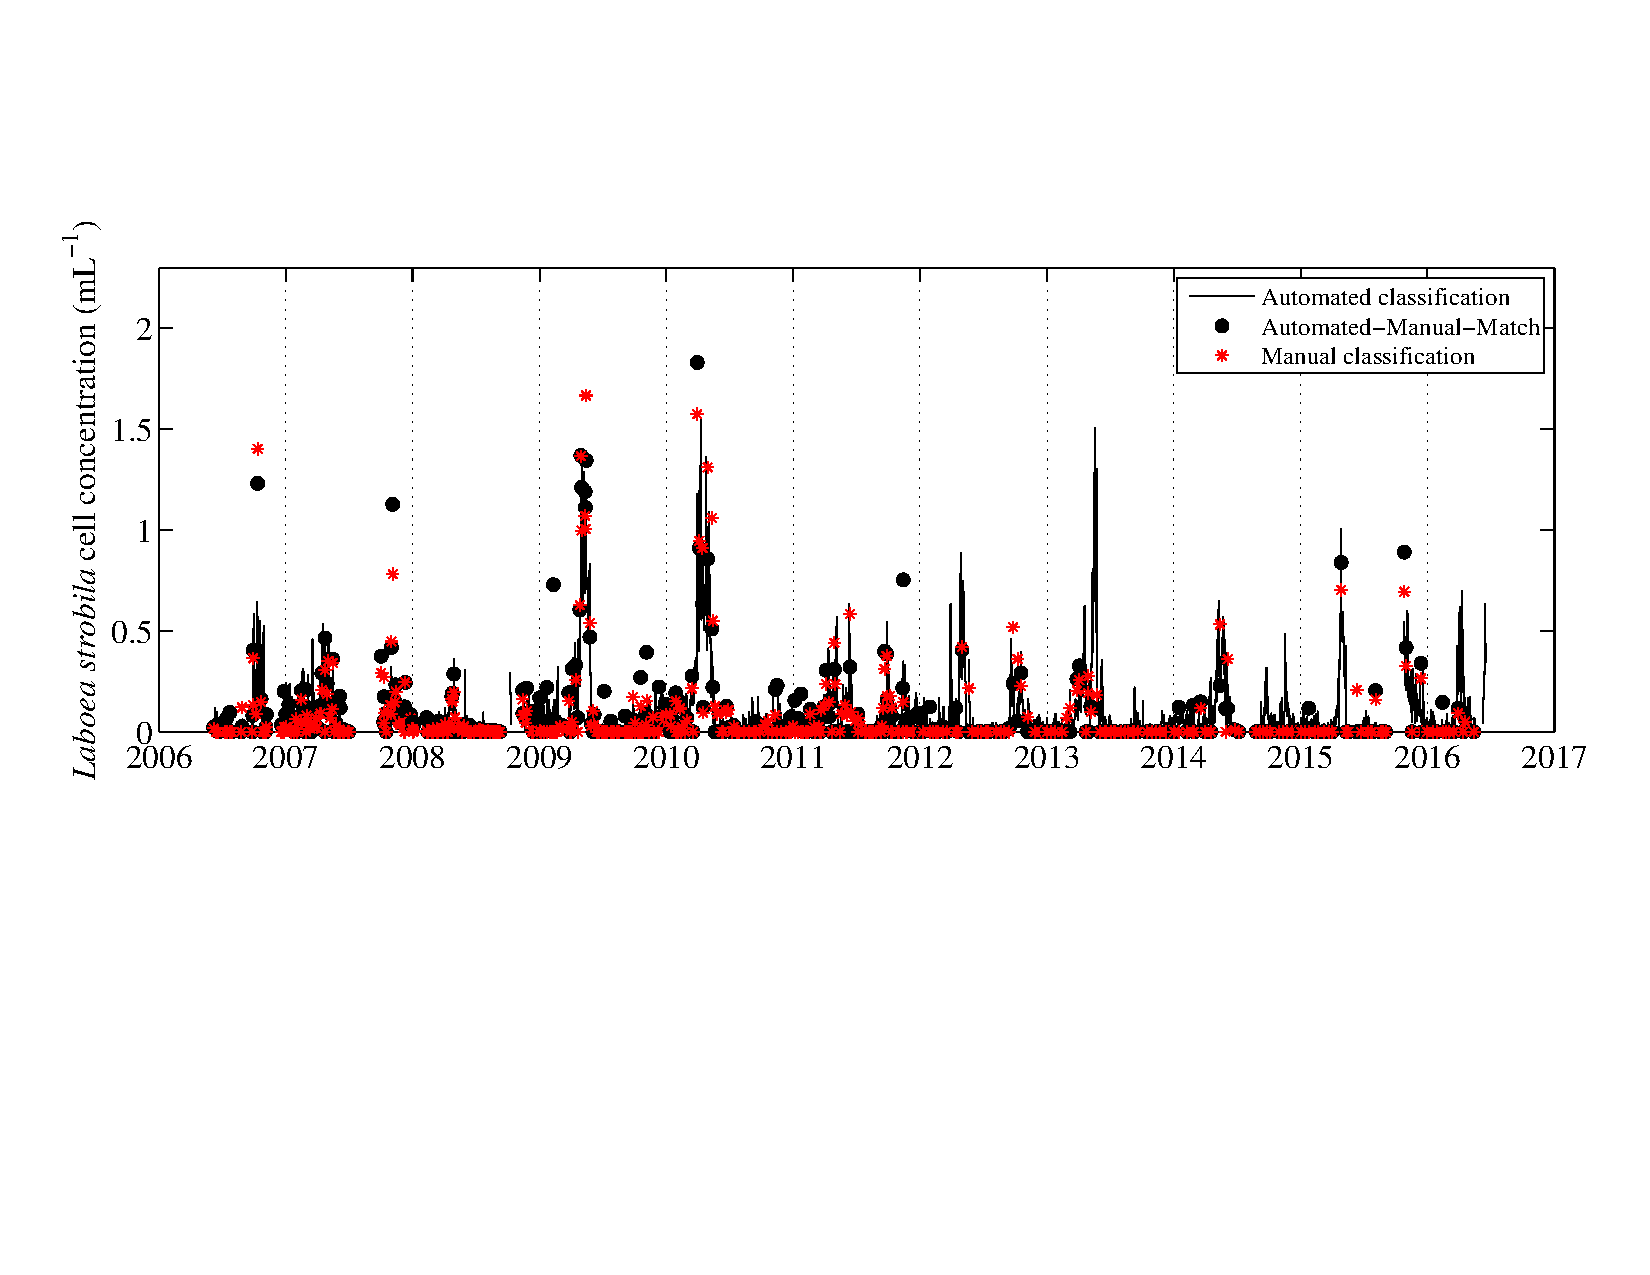
\includegraphics[scale=0.7, angle=90]{Laboea_TB_manual_matched.pdf}
\caption [Comparison between automated and manual classification for \textit{Laboea strobila}] {Daily resolution times series of \textit{Laboea strobila} cell abundance at MVCO. Intermittent (approximately 2 wk interval) counts from manual identification (red stars) are shown with the high-resolution results from automated classification (black line). Automated classification results for exact time bin as manual identification are shown with black circles.}
%\label{arm:fig2}
\end{figure}

\graphicspath{ {Chapter3_Figures/} }
\begin{figure}
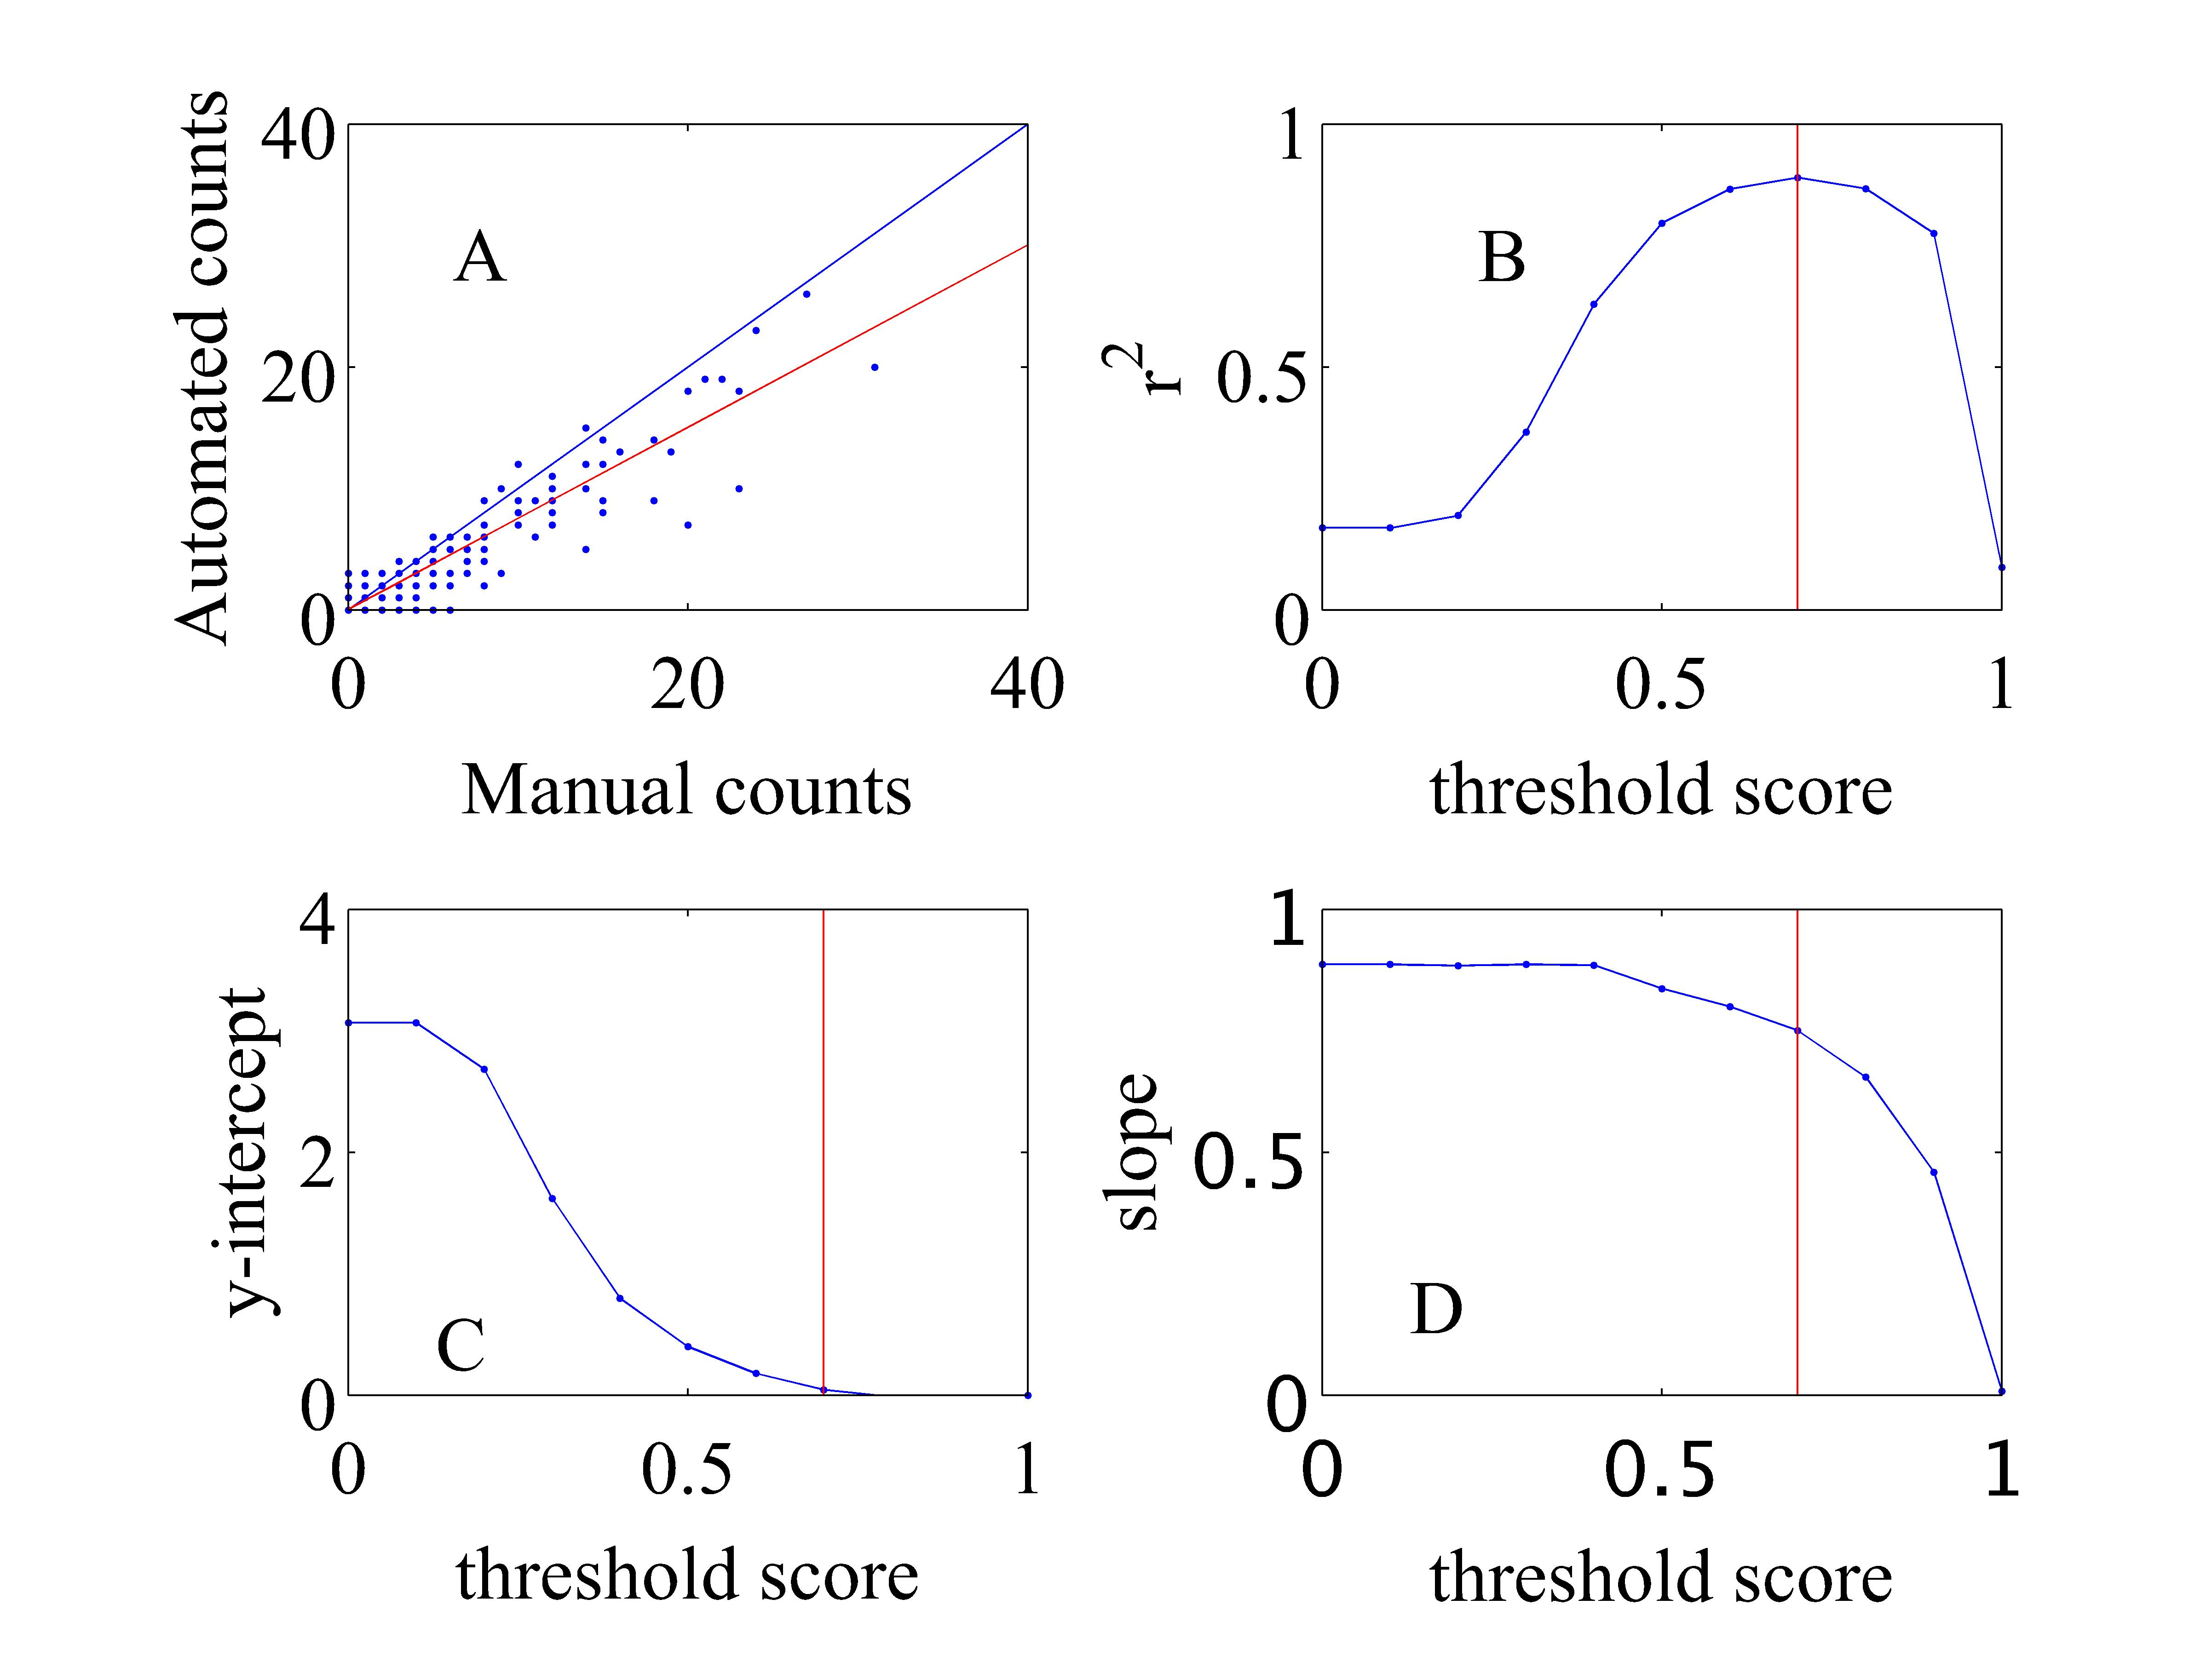
\includegraphics[scale=0.1]{threshold_summary}
\caption [ Indicators for optimal threshold use in automated image classification] {(A) Regression between hourly bins of manually identified  \textit{Laboea strobila} cell abundances at MVCO and automated
classification results for score threshold 0.7. The blue line represents a 1:1 line and the red line is best fit; (B) R$^{2}$ values for all thresholds tested; (C) y-intercept values of best fit line for all thresholds tested; (D) slope values of best fit line for all thresholds tested. Vertical green line in B-D indicates selected threshold score of 0.7}
%\label{arm:fig2}
\end{figure}

\graphicspath{ {Chapter3_Figures/} }
\begin{figure}
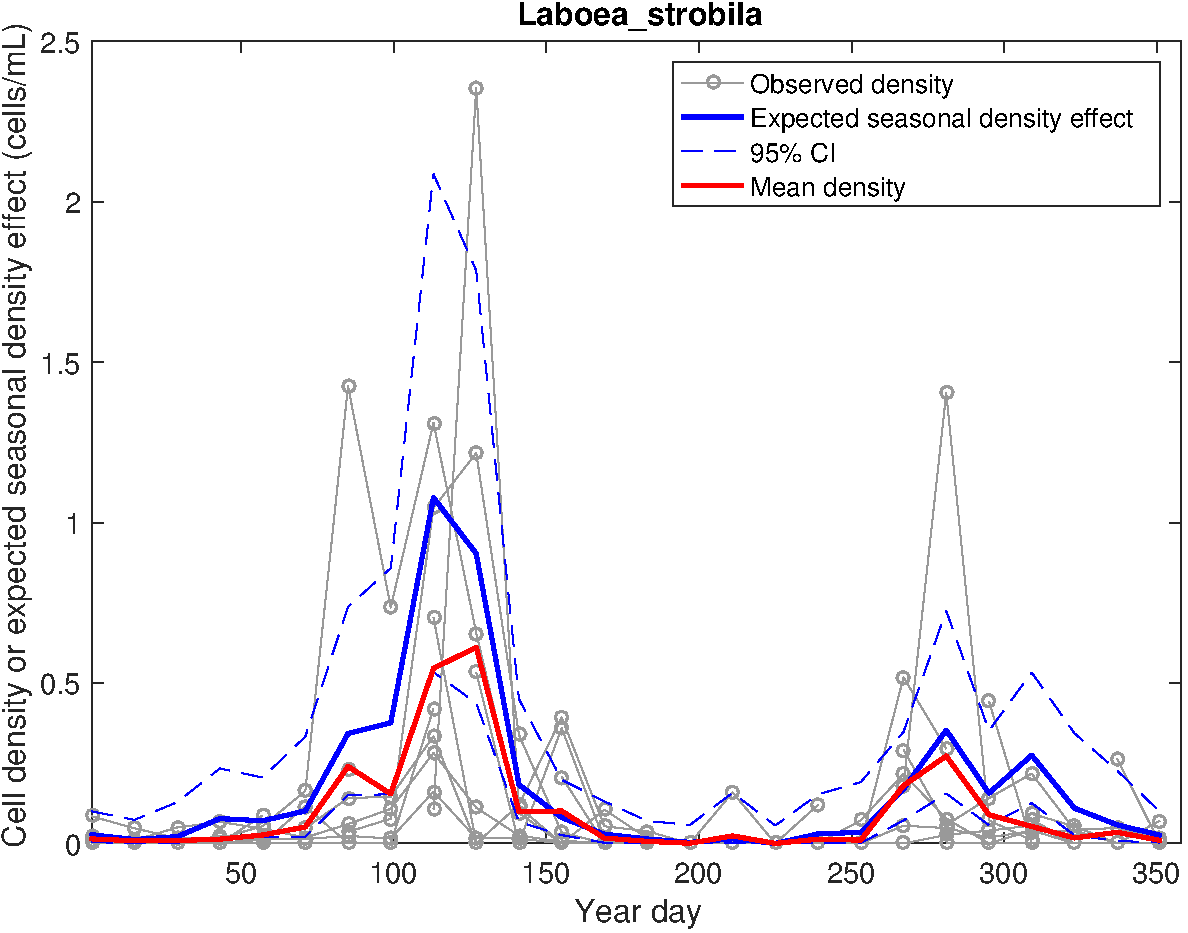
\includegraphics[scale=0.8]{Laboea_summary.pdf}
\caption [\textit{Laboea strobila} climatology] {\textit{Laboea strobila} cell concentration climatology at MVCO. Dotted line indicates 95\% confidence intervals computed assuming Poisson distributed counting statistics.}
%\label{arm:fig2}
\end{figure}

\graphicspath{ {Chapter3_Figures/} }
\begin{figure}
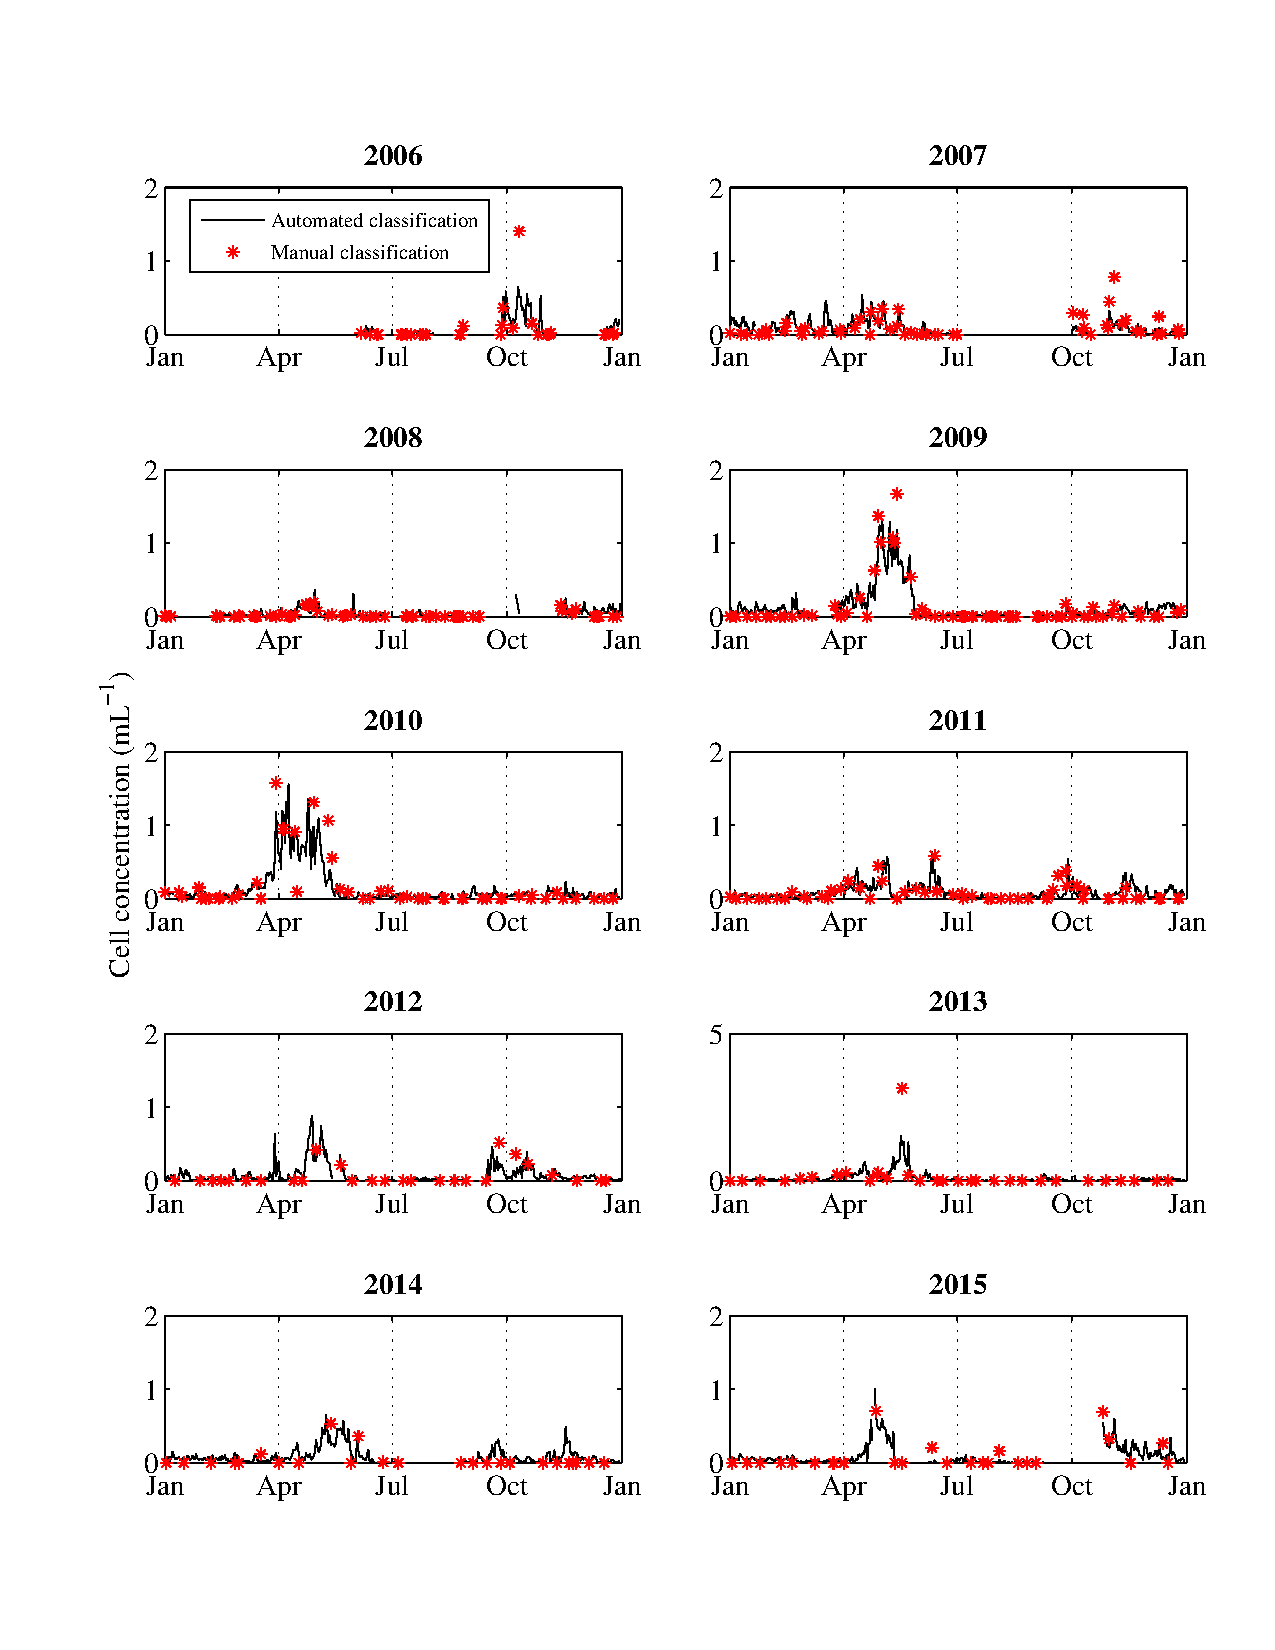
\includegraphics[scale=0.75]{Laboea_automated_vs_manual_byyear.pdf}
\caption [\textit{Laboea strobila} cell concentration and biomass by year] {Daily resolved times series of \textit{Laboea strobila} cell abundance and biomass at MVCO for each year in the timeseries. Intermittent (approximately 2 wk interval) counts from manual identification (red stars) are shown with the high-resolution results from automated classification (black line).}
%\label{arm:fig2}
\end{figure}

\graphicspath{ {Chapter3_Figures/} }
\begin{figure}
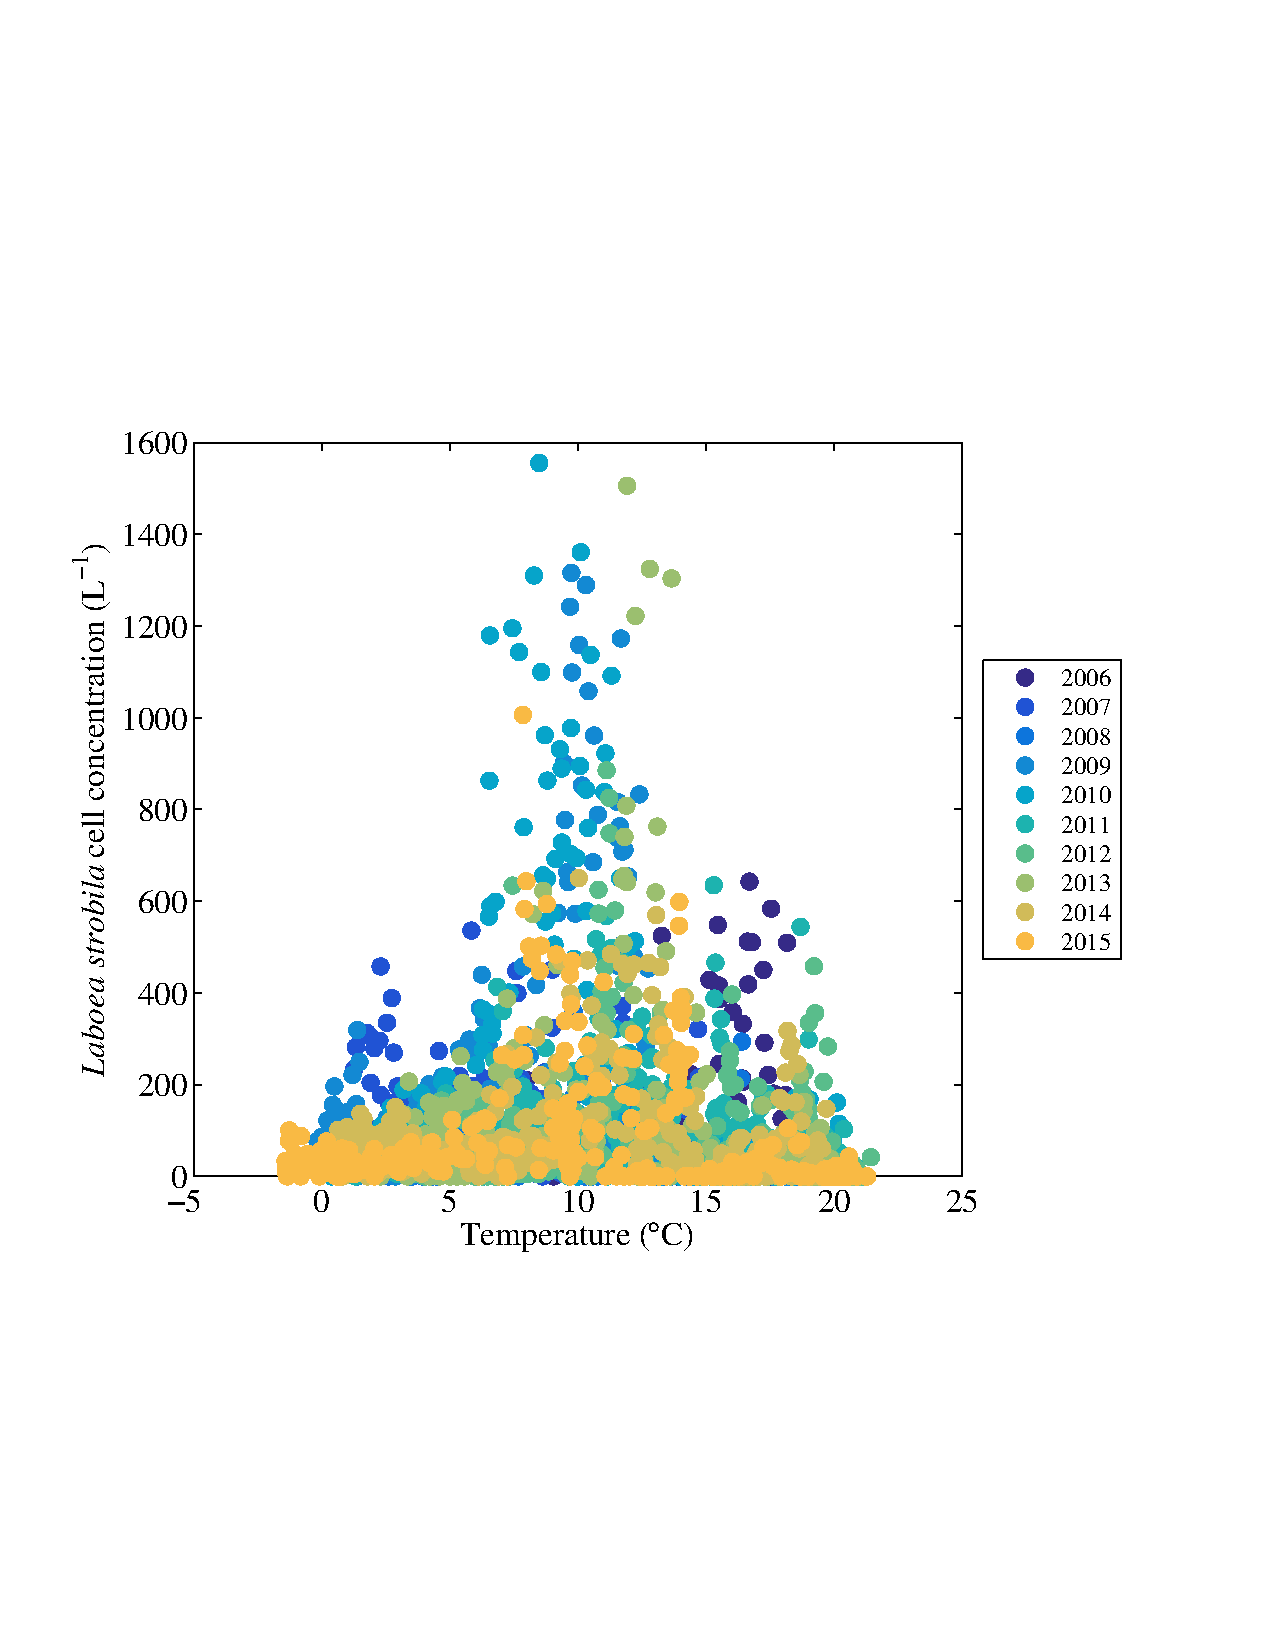
\includegraphics[scale=0.8]{Laboea_Counts_vsTemperature_automated.pdf}
\caption [Relationship between \textit{Laboea strobila} and temperature] {Relationship between of daily resolved automated classification counts for \textit{Laboea strobila} and temperature}
%\label{arm:fig2}
\end{figure}

\graphicspath{ {Chapter3_Figures/} }
\begin{figure}
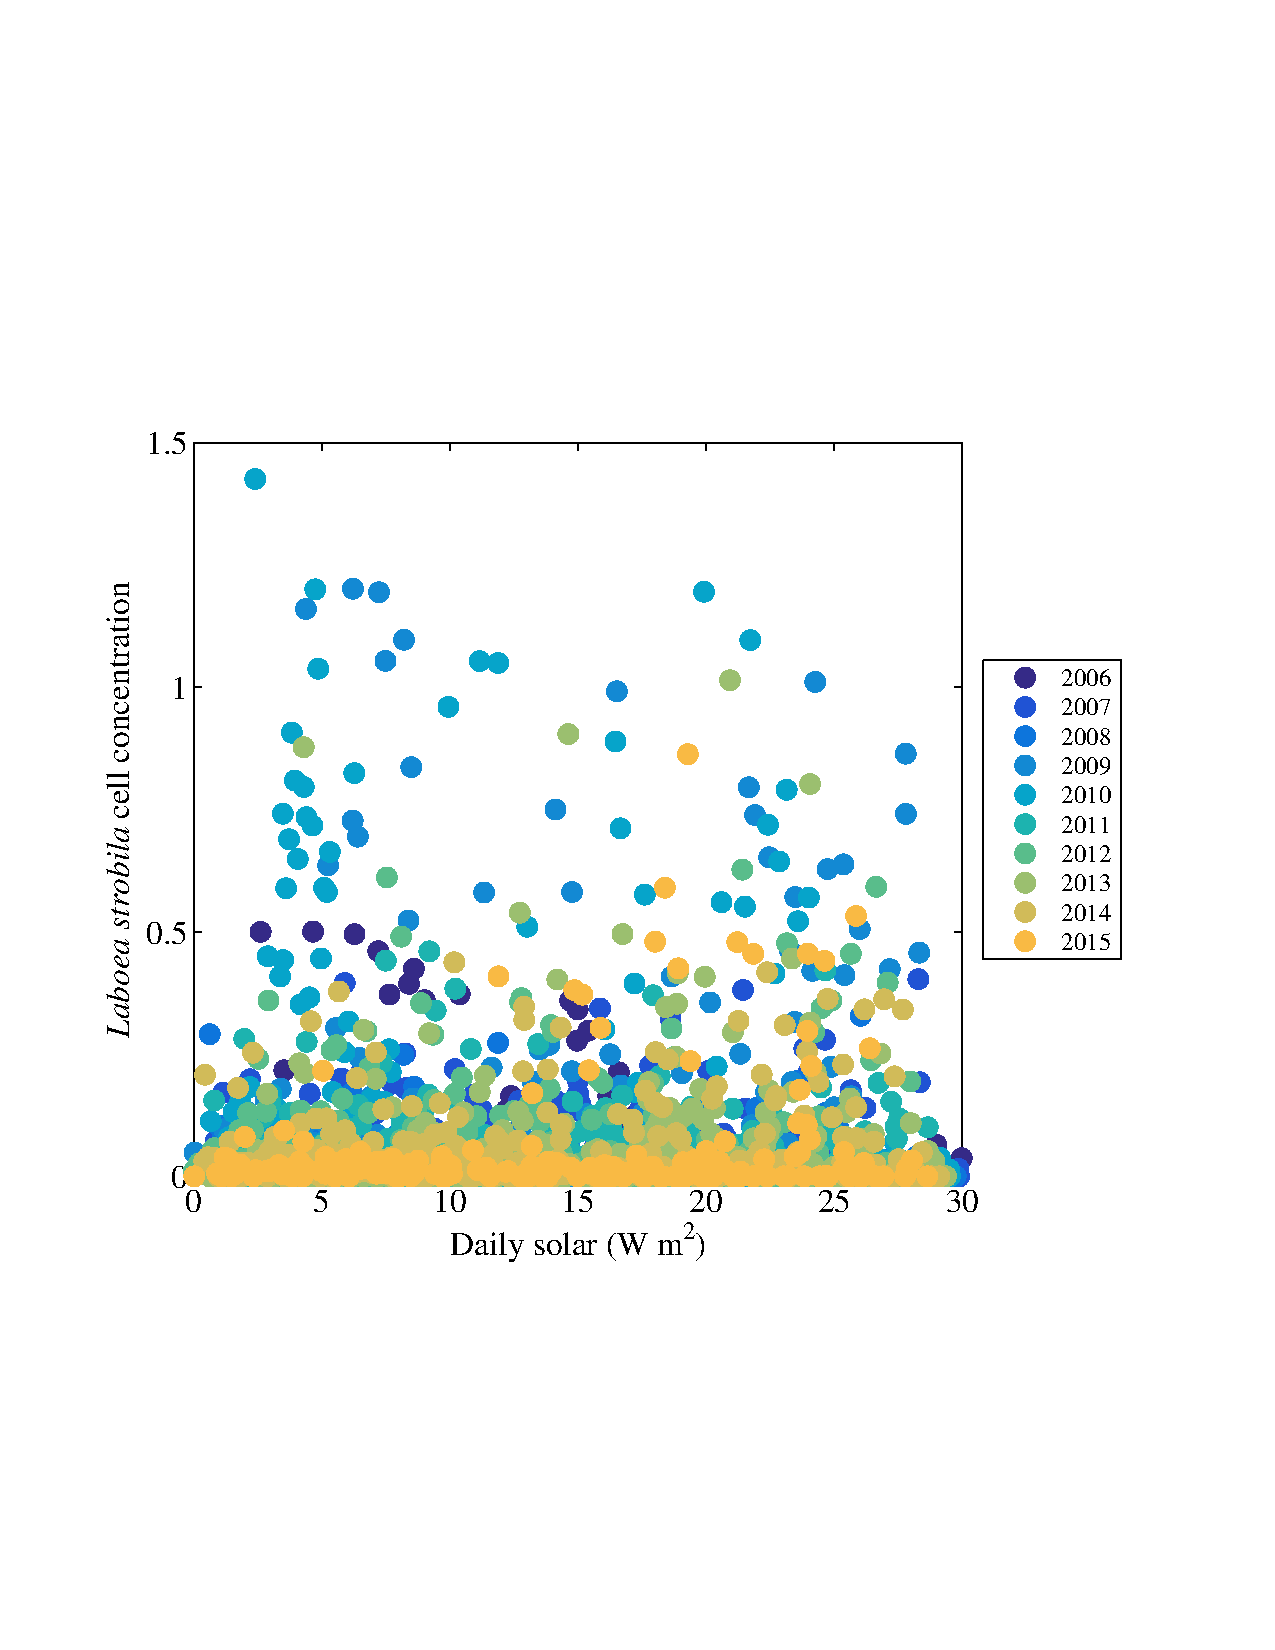
\includegraphics[scale=0.8]{Laboea_Counts_vsDailySolar_automated.pdf}
\caption [Relationship between \textit{Laboea strobila} and solar radiation] {Relationship between of daily resolved automated classification counts for \textit{Laboea strobila} and daily solar radiation}
%\label{arm:fig2}
\end{figure}

\graphicspath{ {Chapter3_Figures/} }
\begin{figure}
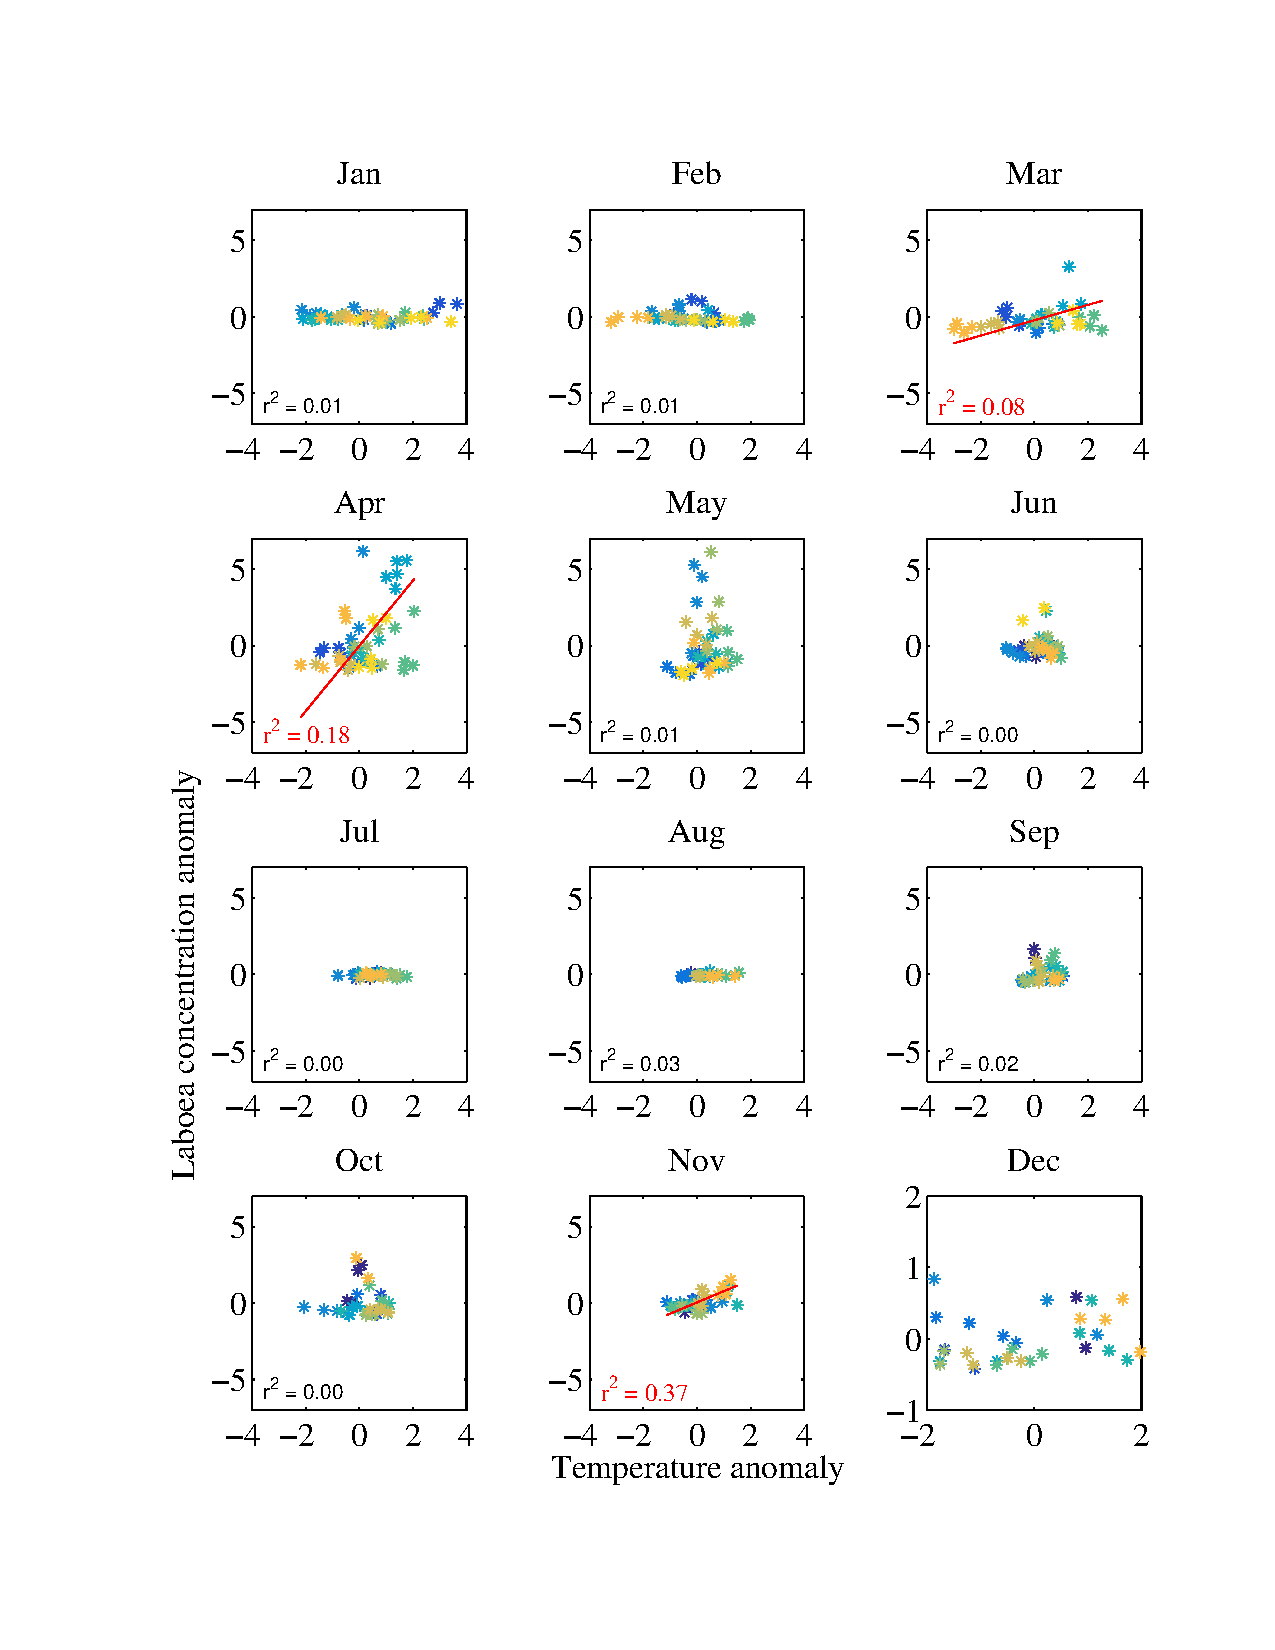
\includegraphics[scale=0.75]{Laboea_anomaly_vs_Temp_TB_allmonths.pdf}
\caption [\textit{Laboea strobila} abundance anomaly vs. temperature anomaly] {Correlation between weekly resolved \textit{Laboea strobila} abundance anomaly with automated image classification and weekly resolved tempurature anomaly by month for the entire time series. Red line indicates the correlation was significant (p <0.05).}
%\label{arm:fig2}
\end{figure}

\graphicspath{ {Chapter3_Figures/} }
\begin{figure}
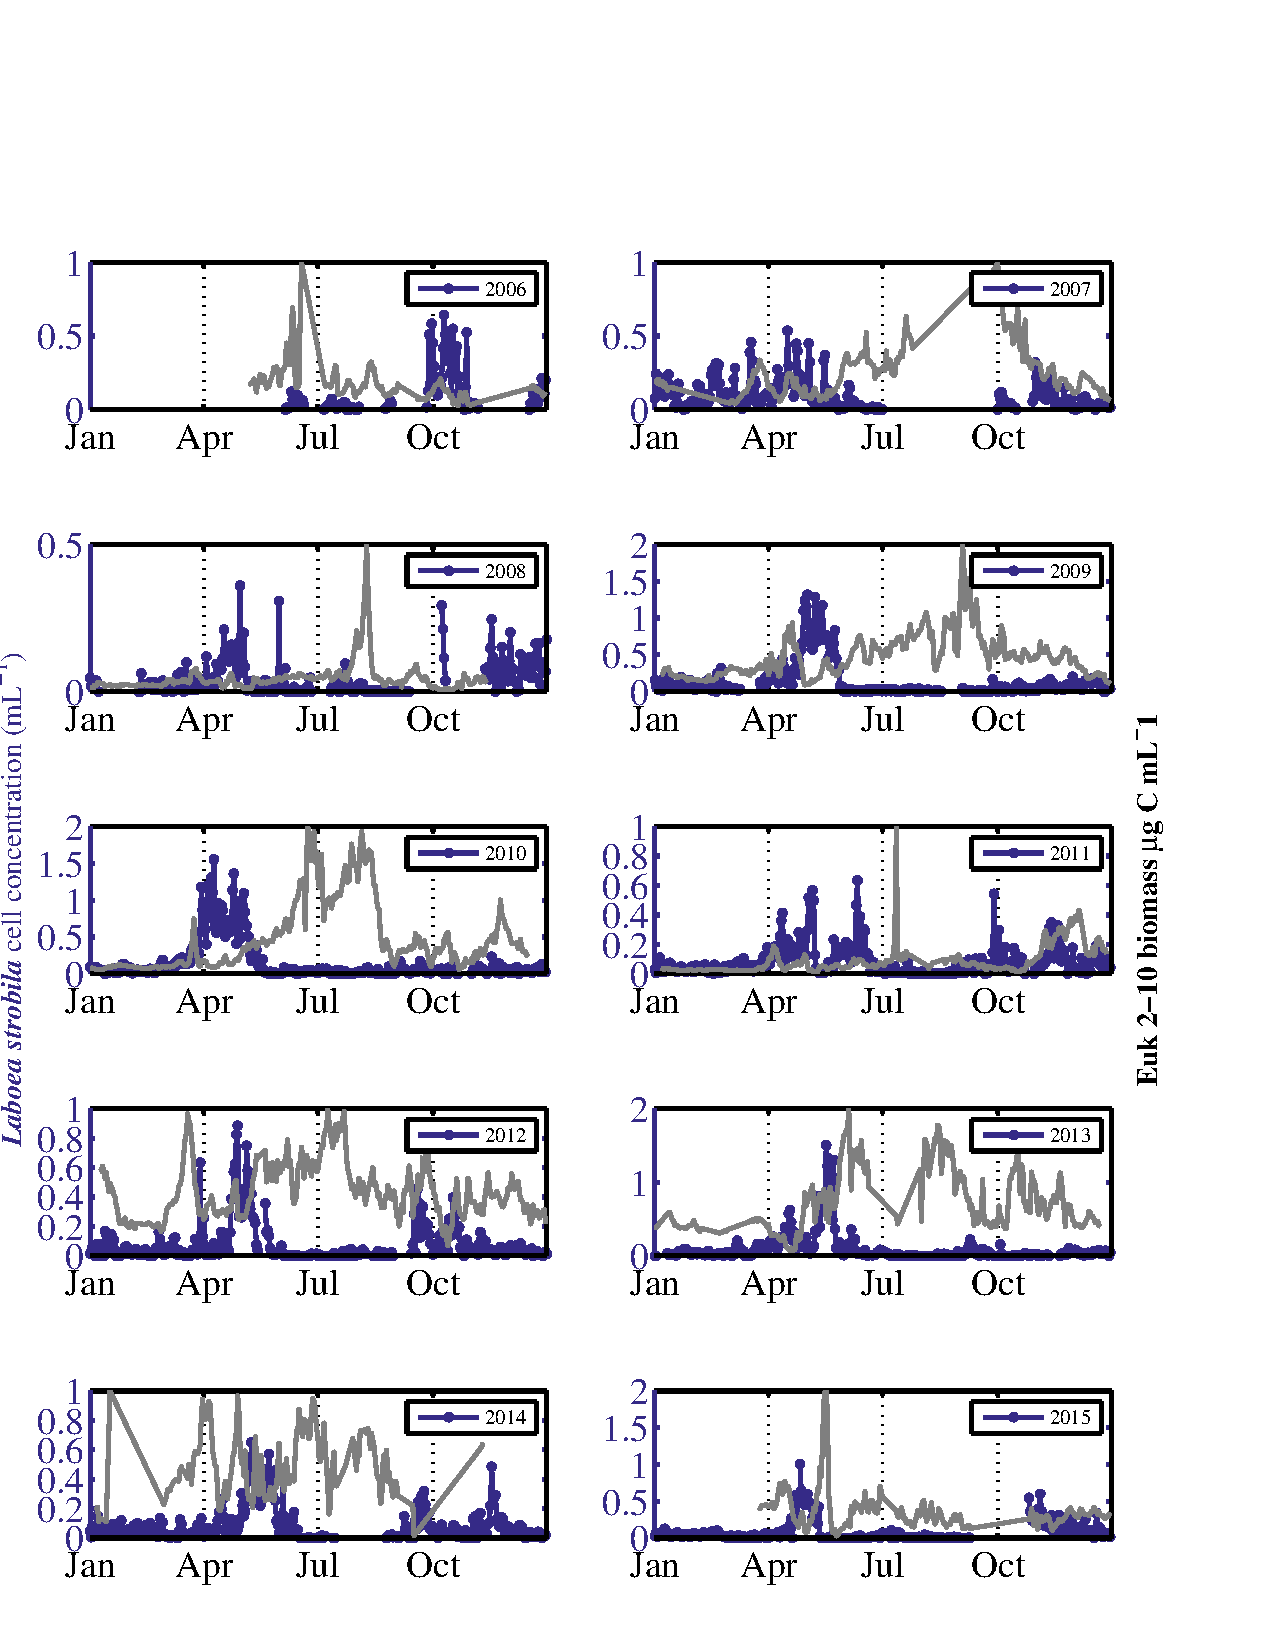
\includegraphics[scale=0.80]{Laboea_counts_vs_EukBiomass.pdf}
\caption [\textit{Laboea strobila} and 2-10 $\upmu$m eukaryote biomass] {Daily resolved times series of \textit{Laboea strobila} cell abundance overlayed with 2-10 $\upmu$m eukaryote biomass for each year in the time series.}
%\label{arm:fig2}
\end{figure}

\graphicspath{ {Chapter3_Figures/} }
\begin{figure}
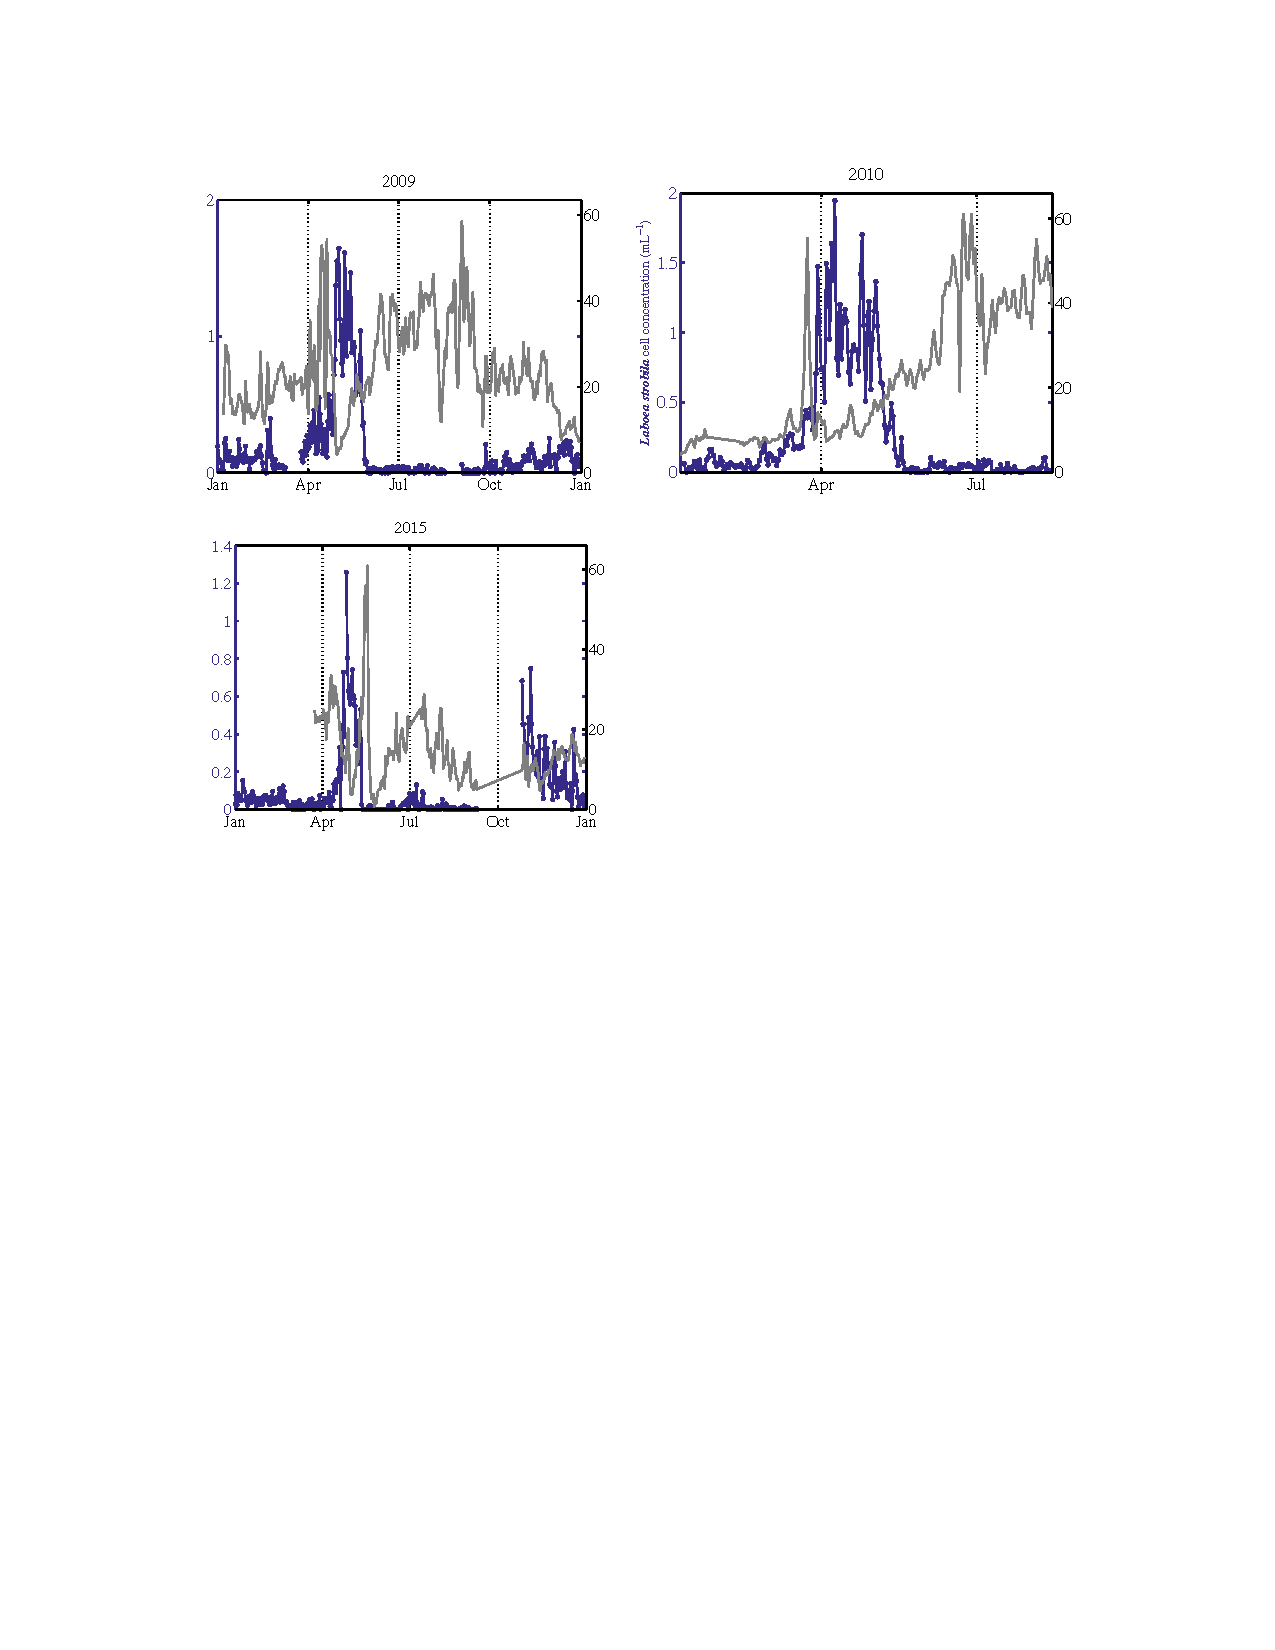
\includegraphics[scale=0.9]{Laboea_euk_panel.pdf}
\caption [Winter and spring \textit{Laboea strobila} and 2-10 $\upmu$m eukaryote biomass] {Daily resolved times series of \textit{Laboea strobila} cell abundance overlayed with 2-10 $\upmu$m eukaryote biomass for each year in the time series from Jan 1-Aug 1}
%\label{arm:fig2}
\end{figure}


